\documentclass{article}
\usepackage{float}
\usepackage[pdftex]{graphicx}
\usepackage{listings}
\usepackage{xcolor}
\lstset{basicstyle=\ttfamily,
  showstringspaces=false,
  commentstyle=\color{red},
  keywordstyle=\color{blue}
}
\begin{document}

\author{Jon Robison}
\title{CS595 Assignment 9}
\maketitle

Q1.\\
Create a blog-term matrix. Start by grabbing 100 blogs.\\
See Appendix A for program to generate bloglist, generateUrls.py\\*

Q2.\\
Create an ASCII and JPEG dendrogram that clusters (i.e., HAC)\\
the most similar blogs.\\
\graphicspath{q1/}
\begin{figure}[H]
  \centering
  \caption{Dendrogram}
  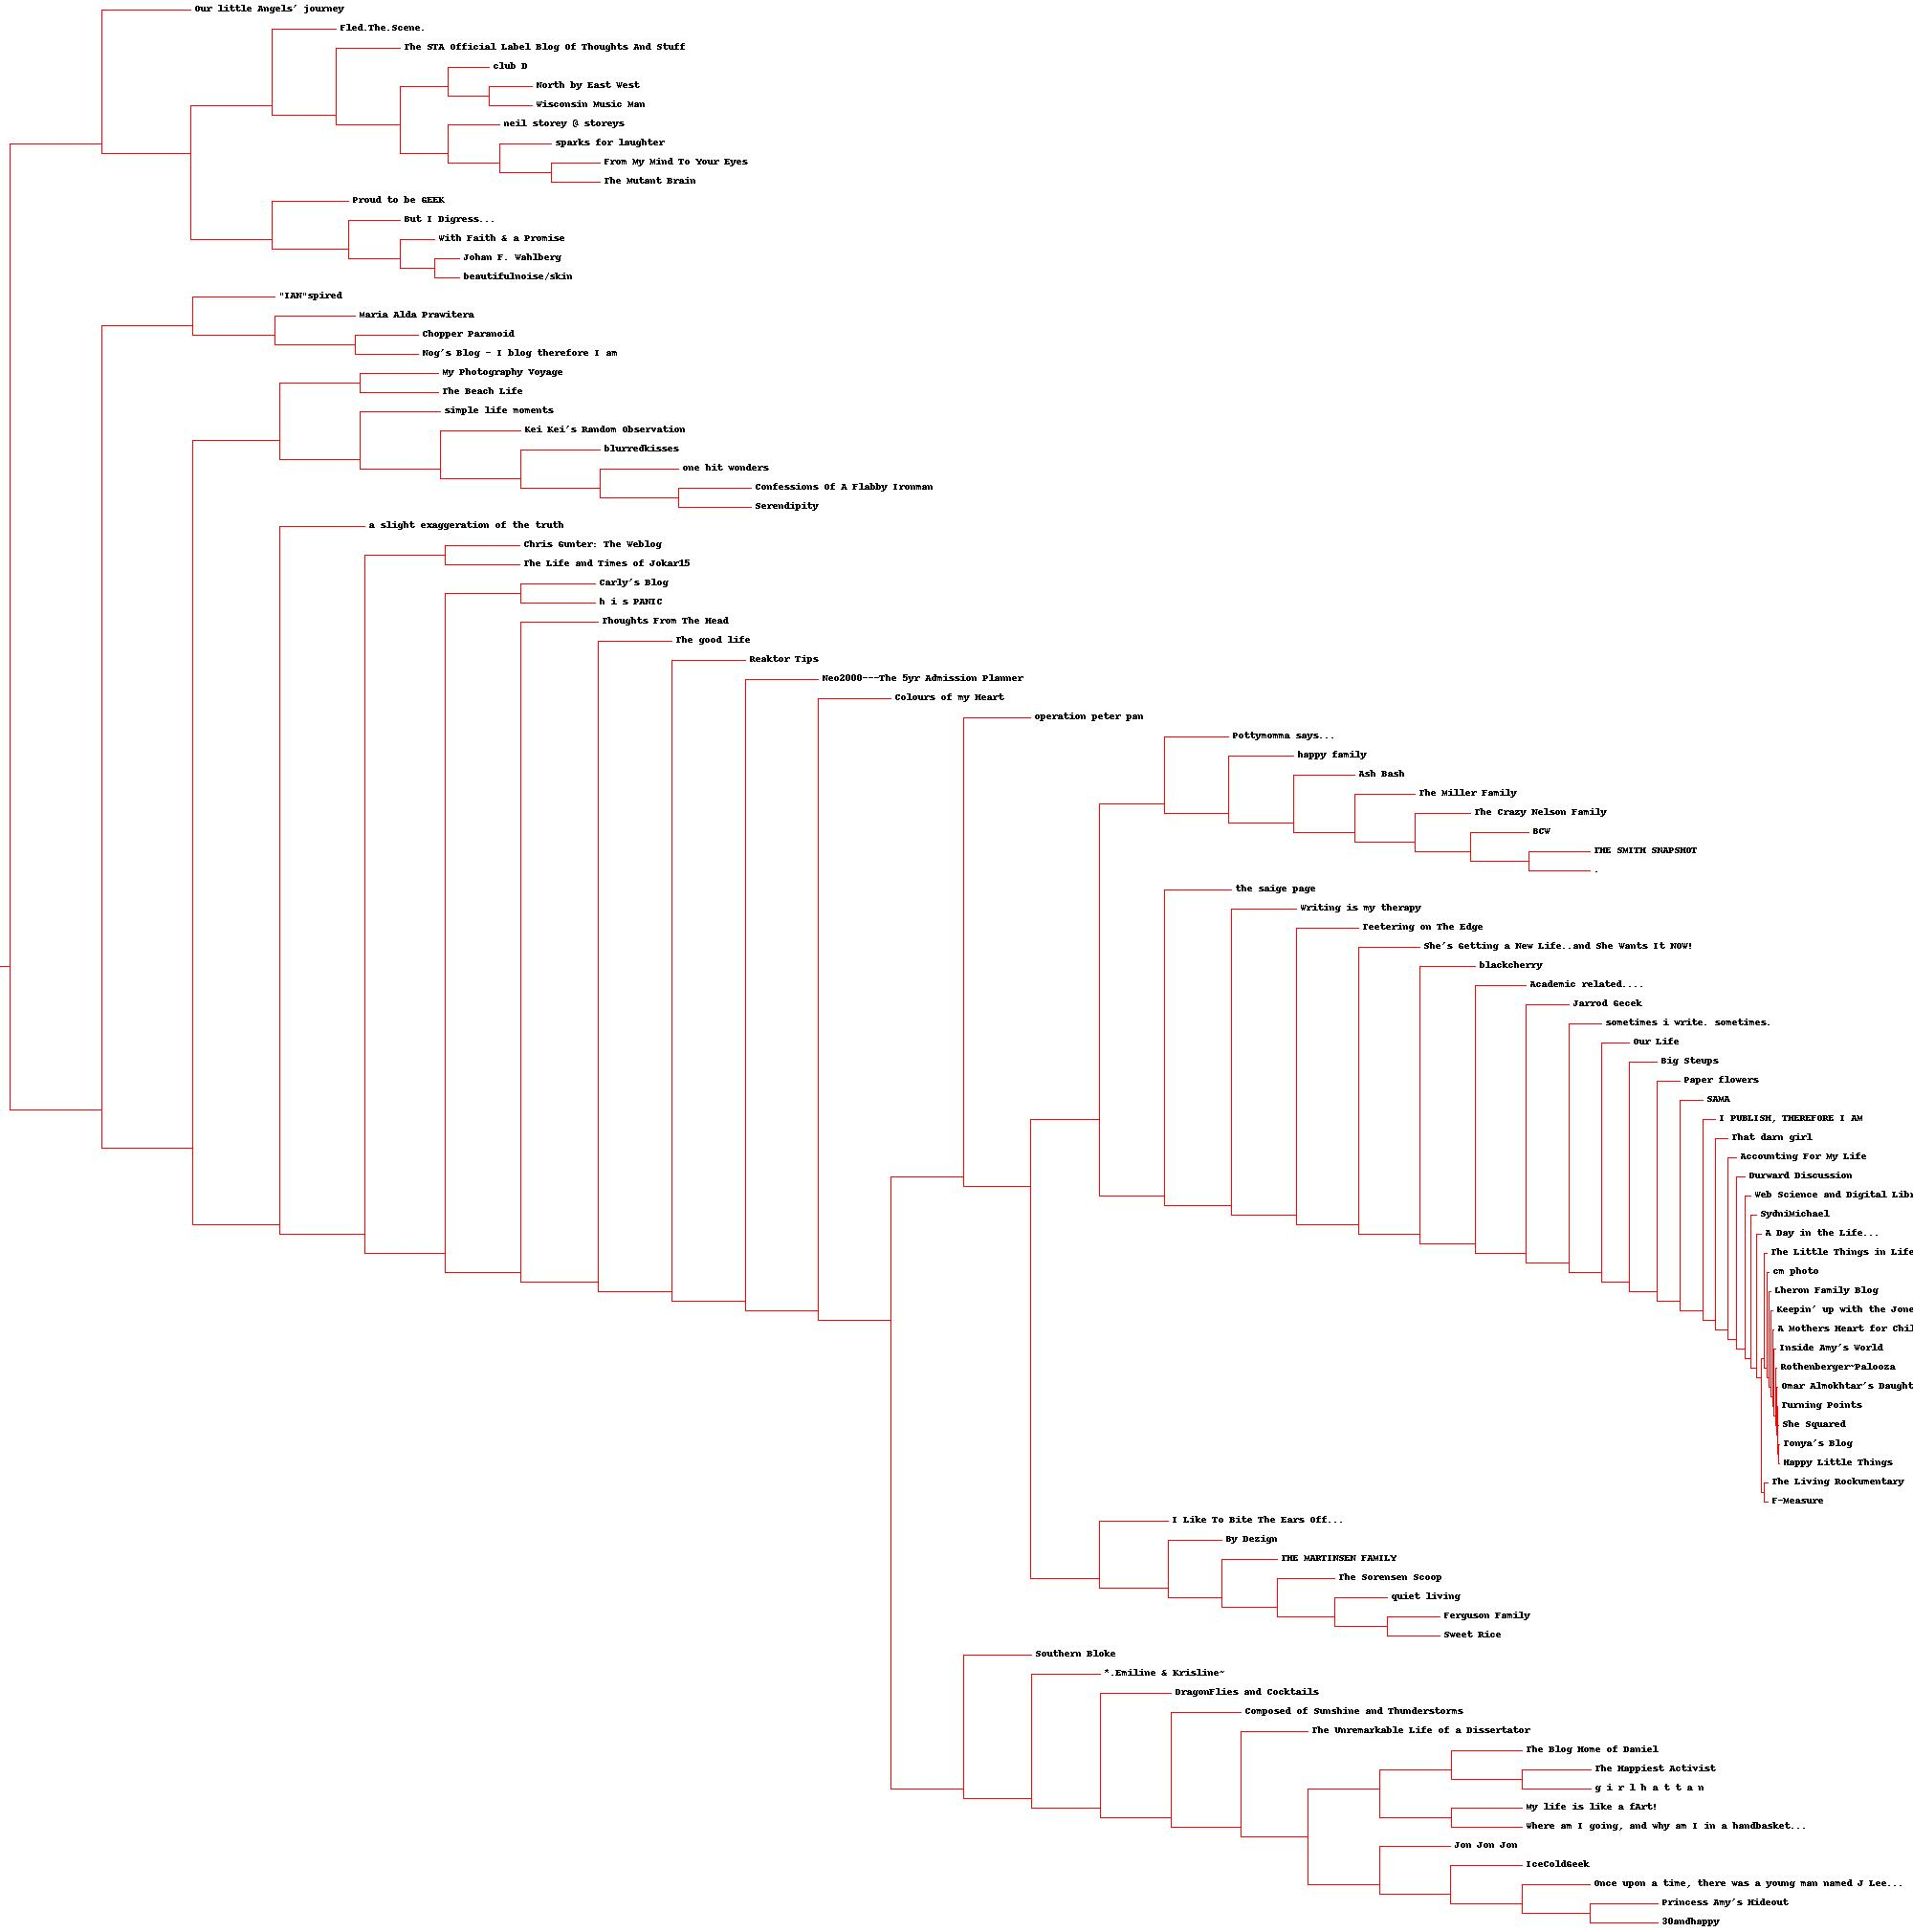
\includegraphics[scale=.5]{dendrogram.jpg}
\end{figure}
\clearpage

Q3.\\
Cluster the blogs using K-Means, using k=5,10,20. (see slide 18).\\
How many interations were required for each value of k?\\
\begin{tabular}{c c}\\
K=5 & 5\\
K=10 & 7\\
K=20 & 7\\
\end{tabular}

Q4.\\
Use MDS to create a JPEG of the blogs similar to slide 29.\\
How many iterations were required?\\

\appendix
\newpage
Appendix A
\lstinputlisting[language=python]{q1/generateUrls.py}
\end{document}
